\documentclass[a4paper]{article}

\usepackage[francais]{babel}
\usepackage[utf8]{inputenc}
\usepackage[T1]{fontenc} 
\usepackage{fullpage}
\usepackage{graphicx}
\usepackage{xspace}

\usepackage{amsmath}
\usepackage{amsfonts}
\usepackage{amssymb}

\usepackage{hyperref}

%% Tikz for picture drawing %%
\usepackage{tikz}
\usetikzlibrary{arrows}

\usepackage{xcolor,colortbl}
\usepackage{tabularx}
\usepackage{caption}
\usepackage{subcaption}
\usepackage{float}
\usepackage{subfloat}

\graphicspath{{figures/}}

\providecommand{\resume}[1]{\textbf{\textit{Résumé---#1}}}
\providecommand{\keywords}[1]{\textbf{\textit{Mots-clés---#1}}}

\newcommand{\TODO}{\textcolor{red}{\textbf{TODO}}}
\newcommand{\AB}{\emph{Alpha-Bêta}}

\newcommand\q[1]{%(question~#1)}
}
\newcommand\qs[1]{%(questions~#1)}
}
\newcommand\C[1]{\texttt{#1}}

\setlength{\parskip}{1em}


\begin{document}


\title{ARCSYS2 Projet 2%
	\\ Communiquer et jouer en réseau}
\author{Simon Bihel, Florestan De Moor%
	 \\ ENS Rennes, 1ère année Département Informatique et Télécommunications}
\date{05 Avril 2016}

\maketitle

\resume{Ce projet consiste à porter le jeu des 7 couleurs sur un serveur. Ainsi, des clients pourront se connecter au serveur pour assister à la partie et la retransmettre, ou bien pour jouer à distance.}\\

\keywords{Serveur ; Client ; Socket ; Réseau}

\section*{Introduction}


Nous avons dans un projet précédent programmé un jeu des 7 couleurs en langage 
\texttt{C}, permettant à des joueurs humains et des joueurs artificiels de 
s'affronter. Nous avions pour cela implémenté différentes stratégies 
utilisables par des intelligences artificielles, et nous avions comparé leurs 
efficacités à travers un tournoi.

Mais tel que nous l'avons implémenté, si deux joueurs humains veulent jouer, 
ils doivent le faire sur la même machine. Si un tiers veut regarder la partie 
en tant que spectateur, il doit être physiquement présent devant l'écran de la 
machine sur laquelle tourne le jeu. Ceci est peu pratique, et ne permet pas une 
diffusion à large échelle des informations.

C'est pourquoi nous allons à travers ce projet modifier notre code source afin 
de le rendre compatible à une utilisation par un réseau. Le but est de faire 
tourner le jeu sur un serveur, et d'avoir des clients qui peuvent se connecter 
au serveur soit pour jouer, soit pour assister au match et le retransmettre.

Dans un premier temps, on s'intéresse à l'ajout de spectateurs, puis on fait jouer des joueurs à distance, et enfin, on modifie le serveur pour qu'il impose des contraintes équitables aux joueurs.

\section{Ajout de spectateurs}

Nous avons récupéré le code du jeu des 7 couleurs écrit par Simon Bihel et Corentin Ferry, qui était très bien documenté, et bien structuré. \\

On va faire tourner le jeu sur un serveur, et ajouter la possibilité pour un client d'assister au match à distance.
On utilise le port 7777 par défaut. \\


Pour assister à un match en cours sur un serveur, on utilise la fonction \texttt{spectate()}. Cette fonction suit les différentes étapes suivantes :

%
\begin{itemize}
	\setlength\itemsep{0.5em}
	\item On ouvre un socket client, et on se connecte au serveur.
	\item On envoie une requête \texttt{SPECTATE\_REQUEST} pour signifier au serveur qu'on se connecte en tant que spectateur.
	\item On reçoit du serveur l'état actuel du jeu, la chaîne de caractère suit le format suivant :

		\bgroup
		\def\arraystretch{1.5}
		\begin{center}
		\begin{tabular}{|c|c|}
			\hline 
			\texttt{board\_size[40]} & \texttt{board[board\_size * board\_size]} \\ 
			\hline 
		\end{tabular} 	
		\end{center}
		\egroup
	
	\item On lance alors une partie qui démarre de la configuration reçue, en local. Le serveur envoie un coup sous la forme d'une chaîne de deux caractères. Le premier est la valeur du coup (donc une couleur), et le deuxième le symbole du joueur jouant ce coup. On met à jour le jeu local selon ces informations, et on affiche l'état courant du jeu. 
	\item Lorsque la partie est détectée en local comme étant terminée, on 
	affiche le résultat final, et le socket client se ferme. \\

\end{itemize}
%


\noindent Côté serveur, le protocole est un peu plus compliqué, puisqu'on veut pouvoir 
gérer potentiellement plusieurs spectateurs, dont certains qui arrivent en 
cours de partie. \\

\noindent Regardons d'abord comment le début d'une partie se déroule.
\begin{itemize}
	\setlength\itemsep{0.5em}
	\item On lance le serveur et attend de recevoir des connections pendant 
	quelques secondes.
	\item Lorsqu'on reçoit une connexion, on l'ajoute à un tableau qui garde en 
	mémoire tous les clients connectés.
	\item À chaque fois qu'on reçoit une connexion, on regarde si on a reçu un 
	message pour demander à regarder la partie (\texttt{SPECTATE\_REQUEST}), si c'est le cas alors on ajoute 
	le dernier client accepté dans un second tableau qui garde en mémoire les 
	observateurs.
	\item Une fois qu'on arrête d'attendre, on lance la partie. D'abord on 
	envoie le plateau initial à tous les observateurs.
	\item Pour chaque coup joué on envoie la couleur jouée ainsi que le 
	l'identifiant du joueur qui vient de jouer. \\
\end{itemize}

%
\begin{figure}[H]
	\centering
	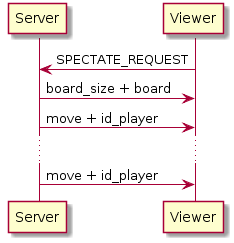
\includegraphics[scale=0.6]{viewer.png}
	\caption{Protocole spectateur}
\end{figure}
%

\noindent Pour avoir des observateurs qui arrivent en milieu de partie, à chaque fois
qu'on envoie le coup qui vient d'être joué aux observateurs, on voit s'il y a
une connexion en attente et si ce nouveau client veut regarder la partie. Si c'est le cas, alors 
on l'ajoute au tableau des observateurs et on lui envoie l'état actuel du
plateau. \\

On peut ainsi avoir plusieurs spectateurs, qui peuvent arriver n'importe quand pendant le jeu. On effectue des tests en local avec l'adresse 127.0.0.1, en lançant plusieurs processus dans différents terminaux. On commente le code, et on génère la documentation avec \emph{Doxygen}.


\section{Joueurs à distance}

\subsection{Faire jouer des clients}

On souhaite avoir un client qui peut jouer au jeu à distance en se connectant au serveur. On suit le schéma suivant :

%
\begin{itemize}
	\setlength\itemsep{0.5em}
	\item Le client envoie au serveur un code spécifique signifiant qu'il veut jouer, c'est une requête pour jouer (\texttt{PLAY\_REQUEST}).
	\item Il reçoit la réponse du serveur. Si c'est non (typiquement si la partie est déjà commencée, où s'il y a déjà deux joueurs), alors la demande est refusée, et le client est basculé en mode spectateur. Si la réponse est oui, la demande est acceptée, et le serveur a enregistré le client comme étant joueur.
	\item Le client reçoit une demande de stratégie du serveur. Il choisit sa stratégie, et l'envoie au serveur.
	\item Le serveur envoie ensuite le tableau initial du jeu, pour commencer à jouer.
	\item Le serveur envoie au client l'information suivante : est-ce que le client joue en premier ou non ?
	\item Le jeu tourne sur le serveur. Lorsque c'est au tour du joueur distant 
	de jouer, le serveur attend automatiquement le coup du joueur. De son côté, 
	le client fait tourner en local un jeu afin de pouvoir calculer son coup 
	suivant, et il l'envoie au serveur.
	%, et celui-ci envoie des requêtes de coup au client lorsque c'est 
	%nécessaire. Le client fait tourner en local un jeu afin de pouvoir 
	%calculer 
	%son coup suivant, et il l'envoie au serveur. \TODO
	\item Le serveur envoie au client les coups de l'adversaire, pour qu'il puisse mettre à jour sa version locale du jeu.
\end{itemize}
%

%
\begin{figure}[H]
	\centering
	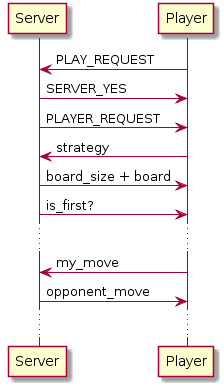
\includegraphics[scale=0.6]{playeryes.png} \hspace{1cm}
	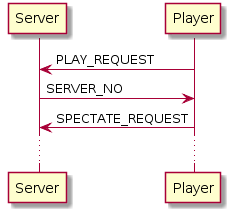
\includegraphics[scale=0.6]{playerno.png}
	\caption{Protocole joueur à distance, selon la réponse du serveur}
\end{figure}
%


\subsection{Robustesse}

Il est possible que lors d'une partie, un joueur déconnecte soudainement ou 
bien que le serveur tombe en panne. Il faut ainsi ajouter des protocoles de 
protection pour savoir comment réagir dans ces cas là.

Si un spectateur déconnecte pendant la partie, le serveur ne doit pas être 
perturbé. Il peut cependant signaler par un affichage qu'il a remarqué une 
déconnexion d'un spectateur.
Plusieurs nouveaux spectateurs peuvent être acceptées à chaque tour du jeu. On accepte un nombre maximum de spectateurs, fixé au départ.
Ainsi, on ne peut pas faire crasher le serveur en envoyant une infinité de spectateurs. \\

Si un joueur déconnecte, le serveur va fermer dès qu'il voudra lui envoyer un message. \\

Du point de vue de la partie client, toutes les interactions avec le serveur 
(avec les fonctions \texttt{send} et \texttt{recv}) sont cachées derrière deux 
fonctions \texttt{server\_to\_client} et \texttt{client\_to\_server}. Ces 
fonctions vérifient la valeur de retour, et utilisent une boucle 
\texttt{while}. Un compteur est initialisé à \texttt{MAX\_SERVER\_MISS} et un 
temps d'attente à une seconde. Si on ne reçoit rien de valide du serveur 
(valeur de retour négative ou nulle), on décrémente le compteur, on attend, et 
on double la valeur du temps d'attente, avant d'entrer dans la prochaine 
itération de la boucle. Obtenir une réponse positive du serveur fait sortir de 
la boucle. Une fois le compteur nul, on sort de la boucle, et on quitte le 
programme en expliquant que le serveur semble être déconnecté. On effectue 
ainsi \texttt{MAX\_SERVER\_MISS} demandes au serveur, espacées d'un temps qui 
augmente exponentiellement. Concrètement, cela signifie que si l'on a pas 
réussi à avoir de connexion avec le serveur au bout de 
$2^{\texttt{MAX\_SERVER\_MISS}} - 1$ secondes, alors on le considère déconnecté. \\

Pour tester la robustesse de notre programme, nous avons effectué des tests en local sur une unique machine,
et également des tests sur trois machines en même temps (nous remercions Louis Béziaud pour sa participation aux essais)
sur lesquels ont tourné en même temps un serveur, un joueur distant et une centaine de spectateurs.
Les résultats nous ont permis d'affiner la robustesse, jusqu'à arriver à des résultats satisfaisants.


\subsection{Limite de temps}

Une limite de temps pour le joueur distant a aussi été implémentée. Côté 
serveur, on attend 5 secondes pour recevoir le coup du joueur distant et si 
aucun coup n'a été reçu, alors on joue à sa place. Après avoir joué à sa place, 
on envoie le coup choisi au joueur distant.

Côté joueur distant, on utilise un \texttt{fork}. Dans le processus fils on 
lance le calcul du prochain coup (algorithme alpha-beta ou demande d'input par 
exemple). Une fois le calcul fait, on pause le processus infiniment. Dans le 
processus père, on attend 5 secondes en vérifiant régulièrement si le coup a 
été calculé. Une fois qu'on a attendu 5 secondes ou que le coup a été calculé, 
on tue le processus fils. Ensuite, si le coup a été calculé, on envoie le coup 
au serveur, sinon il est déjà trop tard et on attend de recevoir le coup qui a 
été joué à notre place par le serveur.

Concernant la chronométrage des deux joueurs, on prend le temps avant de 
lancer/demander le coup suivant et on reprend le temps une fois qu'on a le 
coup. La différence des deux donne le temps pris, et additionne au fil des 
tours. On a utilisé des \texttt{struct timeval} et la fonction 
\texttt{gettimeofday} pour avoir le temps écoulé depuis l'Epoch.



\section{Critique}

Actuellement, on est parti d'une version locale du jeu de 7colors en ajoutant
des interactions serveur/client(s) dans le déroulement d'une partie. Cela peut
encore marcher pour un serveur qui fait une seule partie d'un jeu simple.
Cependant si le jeu avait besoin de plus d'interactions, une mauvais ordre dans
les messages incapaciterait le client. Côté serveur il serait impossible de
gérer plusieurs parties sans avoir des dépendances entre elles. Il faudrait donc
séparer interactions réseaux et jeu. Il y aurait donc un thread dédié au réseau,
et un thread par partie du jeu. Au final le déroulement d'une partie ne serait
rien d'autre qu'un automate. Pour la gestion réseau on pourrait avoir une queue
pour stocker un certain nombre de messages et les traiter dans un ordre
approprié. On pourrait aussi avoir un thread en plus pour ne faire qu'écouter et
mettre les messages dans la queue. Chaque partie aurait un identifiant et chaque
message contiendrait un identifiant pour connaitre son rôle facilement. Il
faudrait un moyen de définir quels messages sont attendus pour permettre à
l'automate/thread de jeu de dormir et de ne le réveiller que lorsqu'un élément
fait avancer la partie.


Pour le joueur distant il faudrait attendre une demande du serveur pour choisir 
une couleur avant de lancer les calculs et envoyer le coup effectué.

On pourrait améliorer la robustesse de notre serveur en essayant de contrer des 
attaques par déni de service (DoS). On pourrait par exemple utiliser 
l'algorithme du CountMin Sketch que nous avons programmé lors d'un projet en 
module d'IRESI.


\section*{Conclusion}

Nous avons donc programmé un serveur sur lequel tourne le jeu des 7 couleurs. 
Des clients ont la possibilité de se connecter au serveur, soit pour jouer, 
soit pour assister au match et le retransmettre. Pour l'instant, la possibilité 
de jouer à distance n'est offerte qu'à un seul joueur. On pourrait modifier le 
programme pour avoir deux joueurs distants. Par ailleurs, le programme est 
fonctionnel pour un round, on pourrait sans difficulté l'adapter pour un 
tournoi, en réinitialisant les joueurs distants et les spectateurs à chaque 
nouveau round. Enfin, on pourrai améliorer le protocole afin d'améliorer les 
performances et la robustesse du serveur.


\bibliographystyle{plain} 
\bibliography{report_arcsys2p2}

\end{document}